\section{The Church of John}

\begin{wrapfigure}{rt}{.35\textwidth}
 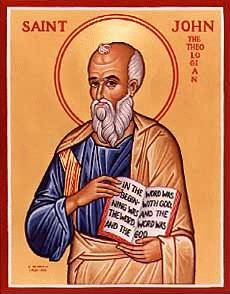
\includegraphics[scale=.5]{a20221120TheChurchofJohn-img001.jpg} 
\end{wrapfigure}

At the end of his Gospel, John
mentions that Peter was questioning Jesus’ relation with John. Jesus replied bluntly, “What's
it to you?”

In Meditations on the Tarot, \textbf{Valentin Tomberg} brings up the often-made distinction between the Church of Peter
and the Church of John, the former structured and hierarchical, the latter free and mystical. Someone asked me the
question: “Does the Roman Catholic Church need Hermetism?” To answer properly, the question needs to be adjusted: “Does
the Church of Peter need Hermetism?” and the answer to this question is “certainly not”.

The real question is really about the Church of John, and there are several questions: “Does it even exist, has it
existed continuously, is its core Hermetism?”

According to the theologian \textbf{Hans Ur von Balthazar}, it does exist\footnote{\emph{The von Balthazar Reader}, \#66},
although he calls the two churches “Official Church” and “Church of Love”, and its source can be found in the Gospel of
John. He says there is a two-peaked church in harmonious tension, although the Church of John respectfully gives
precedence to the Church of Peter. There are no clear boundaries between the two. This interesting discussion concludes
with this:

\begin{quotationx}
Between these two impossible ecclesiologies, the Gospel of John leaves and dismisses us in a suspended middle point
whose foundation lies solely with the Lord. The last thing said to the servant Peter, the last word of the Lord in the
gospel, is the admonition (for the church and theology of all times), “What's it to you?”

\end{quotationx}
So the Church of John exists and has existed continuously. The next question is about Hermetism. There have been many
clues about this. \textbf{Dionysius}, \textbf{Clement of Alexandria}, \textbf{Origen} are close to Hermetism. There
were the alchemists, \textbf{Ramon Lull}, \textbf{Ficino}, \textbf{Louis-Claude de Saint-Martin} … all clues that
Hermetism has always existed in the Church and only occasionally makes a public appearance.

\textbf{Rene Guenon} claims that the Church used to have an esoteric teaching which he claims was Hermetism. He points
to Dante as a member of an esoteric order, and even Thomas Aquinas. The Templars, the Grail Legend, the story of the
Magi, Medieval Romances, St Bernard of Clairvaux, Ramon Lull, Michael Scott, and so on, all point to the existence of a
Christian esoterism. In \emph{Perspectives on Initiation}, Guenon writes in a similar vein about a dual church:

\begin{quotationx}
Within a single organization, a kind of double hierarchy can exist, especially when the apparent leaders are themselves
unaware of any link to a spiritual center. In such cases there may exist beside the visible hierarchy made up by those
apparent leaders, an invisible hierarchy of which the members may not fulfill any `official’ function but who, by their presence alone, nonetheless assure an effective liaison with this center. In the more
exterior organizations these representatives of the spiritual centers obviously need not reveal themselves as such …

\end{quotationx}
Tomberg and van Balthazar agree on the Church of John. It is not separate from the Church of Peter on which it depends
for structure and support. Rather it is a less formal entity, in parallel with, yet not opposed to, the official
church. Historically, there have been times they got along, and other times in opposition. With the destruction of the
Templars, came the Rosicrusians who found themselves opposed to the Church. Then other Hermetists, such as Cagliostro,
Giordano Bruno, or Thomas Campanella were imprisoned and even executed.

Yet to create a visible Church of John with its own separate structure, clergy, doctrine, and so on is, in my opinion, a
mistake; actually I believe it to be impossible. That is because it will eventually degenerate into a vacuous,
undifferentiated, and amorphous entity, not holding firm to anything in particular. As a witness to that, we need only
point to the various so-called New Age and occult movements active today.

The Church of John is in your heart and mind, especially when you are joined with two or three others. So to any
self-appointed guardians of orthodoxy, I ask “What's it to you?”

\flright{\itshape Posted on 2022-11-20 by Cologero 

Originally published on 13 Feb 2011 in medtarot}
